
%%%%%%%%%%%%%%%%%%%%%%%%%%%%%%%%%%%%%%%%%%%%%%%%%%%%%%%%%%%%%%%%%%%%%%%%%%
\section{Intervalo melódico}
\label{sec:intervalomelodico}
\index{Música!Intervalo}
\index{Música!Intervalo melódico}


Um intervalo é a distância que existe entre dois sons de alturas definidas;
os intervalos melódicos correspondem à medição de notas musicais executadas uma após outra, 
numa melodia \cite[pp. 17]{holst1998abc}.
Assim, podem existir intervalos melódicos ascendentes ou descendentes,
que indicam que o tom da nota posterior é mais agudo ou mais grave, respetivamente \cite[pp. 17]{holst1998abc}.

Sobre a unidade de medição que será usada para quantificar as distancias nos intervalos, 
estes podem ser medidos usando sua posição relativa seguindo as sete notas da escala diatônica \cite[pp. 17]{holst1998abc}.
Por exemplo na Tabela \ref{tab:intervalomelodico} podemos ver os nomes usados seguindo esta notação.  
\begin{table}[h]
  \centering
  \begin{tabular}{|l|l||l|l|}
  \hline
  Intervalo & Posição     & Intervalo & Posição \\ \hline \hline
  Uníssono  & 1$^{\circ}$ & Segunda   & 2$^{\circ}$ \\ \hline
  Terça     & 3$^{\circ}$ & Quarta    & 4$^{\circ}$ \\ \hline
  Quinta    & 5$^{\circ}$ & Sexta     & 6$^{\circ}$ \\ \hline
  Sétima    & 7$^{\circ}$ & Oitava    & 8$^{\circ}$ \\ \hline
  \end{tabular}
  \caption{Distancia entre intervalos.}
  \label{tab:intervalomelodico}
\end{table}

Na Figura \ref{fig:abc-isegunda1} podemos ver um intervalo de uma segunda ascendente,
desde um dó até um ré (+2 semitons).
Na Figura \ref{fig:abc-isegunda2} podemos ver um intervalo de uma segunda descendente,
desde um fá até um mi (-1 semitons).
\begin{figure}[H]
    \centering
    \begin{subfigure}[b]{0.4\textwidth}
\begin{abc}[name=abc-isegunda1]
X: 1 % start of header
K: C % scale: C major
V:1 %name="Pauta com clave de fá"   sname="Pauta com clave de fá"
[V:1]  C2 D2
w: ~1º ~2º
\end{abc}
\caption{Intervalo de uma segunda ascendente.}
\label{fig:abc-isegunda1}
    \end{subfigure}
    \quad%~%add desired spacing between images, e. g. ~, \quad, \qquad, \hfill etc. 
      %(or a blank line to force the subfigure onto a new line)
    \begin{subfigure}[b]{0.4\textwidth}
\begin{abc}[name=abc-isegunda2]
X: 1 % start of header
K: C % scale: C major
V:1 %name="Pauta com clave de fá"   sname="Pauta com clave de fá"
[V:1]  F2 E2
w: ~1º ~2º
\end{abc}
\caption{Intervalo de uma segunda descendente.}
\label{fig:abc-isegunda2}
    \end{subfigure}
    \caption{Intervalo melódico de uma segunda.}
    \label{fig:intervalosegunda}
\end{figure}


Na Figura \ref{fig:abc-iterca1} podemos ver um intervalo de uma terça ascendente,
desde um fá até um lá (+4 semitons).
Na Figura \ref{fig:abc-iterca2} podemos ver um intervalo de uma terça descendente,
desde um dó até um lá (-3 semitons) \cite[pp. 16-17]{holst1998abc}.
\begin{figure}[H]
    \centering
    \begin{subfigure}[b]{0.4\textwidth}
\begin{abc}[name=abc-iterca1]
X: 1 % start of header
K: C % scale: C major
V:1 %name="Pauta com clave de fá"   sname="Pauta com clave de fá"
[V:1]  F2 A2
w: ~1º ~3º
\end{abc}
\caption{Intervalo de uma terça ascendente.}
\label{fig:abc-iterca1}
    \end{subfigure}
    \quad%~%add desired spacing between images, e. g. ~, \quad, \qquad, \hfill etc. 
      %(or a blank line to force the subfigure onto a new line)
    \begin{subfigure}[b]{0.4\textwidth}
\begin{abc}[name=abc-iterca2]
X: 1 % start of header
K: C % scale: C major
V:1 %name="Pauta com clave de fá"   sname="Pauta com clave de fá"
[V:1]  |C'2 A2|
w: ~1º ~3º
\end{abc}
\caption{Intervalo de uma terça descendente.}
\label{fig:abc-iterca2}
    \end{subfigure}
    \caption{Intervalo melódico de uma terça.}
    \label{fig:intervaloterca}
\end{figure}



Na Figura \ref{fig:abc-iquarta1} podemos ver um intervalo de uma quarta ascendente,
desde um sol até um dó (+5 semitons) \cite[pp. 17]{holst1998abc}.
Na Figura \ref{fig:abc-iquarta2} podemos ver um intervalo de uma quarta descendente,
desde um sol até um ré (-5 semitons).
\begin{figure}[H]
    \centering
    \begin{subfigure}[b]{0.4\textwidth}
\begin{abc}[name=abc-iquarta1]
X: 1 % start of header
K: C % scale: C major
V:1 %name="Pauta com clave de fá"   sname="Pauta com clave de fá"
[V:1]  G2 C'2
w: ~1º ~4º
\end{abc}
\caption{Intervalo de uma quarta ascendente.}
\label{fig:abc-iquarta1}
    \end{subfigure}
    \quad%~%add desired spacing between images, e. g. ~, \quad, \qquad, \hfill etc. 
      %(or a blank line to force the subfigure onto a new line)
    \begin{subfigure}[b]{0.4\textwidth}
\begin{abc}[name=abc-iquarta2]
X: 1 % start of header
K: C % scale: C major
V:1 %name="Pauta com clave de fá"   sname="Pauta com clave de fá"
[V:1]  G2 D2
w: ~1º ~4º
\end{abc}
\caption{Intervalo de uma quarta descendente.}
\label{fig:abc-iquarta2}
    \end{subfigure}
    \caption{Intervalo melódico de uma quarta.}
    \label{fig:intervaloquarta}
\end{figure}

Na Figura \ref{fig:abc-iquinta1} podemos ver um intervalo de uma quinta ascendente,
desde um si até um fá (+6 semitons).
Na Figura \ref{fig:abc-iquinta2} podemos ver um intervalo de uma quinta descendente,
desde um dó até um fá (-7 semitons) \cite[pp. 17]{holst1998abc}.
\begin{figure}[H]
    \centering
    \begin{subfigure}[b]{0.4\textwidth}
\begin{abc}[name=abc-iquinta1]
X: 1 % start of header
K: C % scale: C major
V:1 %name="Pauta com clave de fá"   sname="Pauta com clave de fá"
[V:1]  B,2 F2
w: ~1º ~5º
\end{abc}
\caption{Intervalo de uma quinta ascendente.}
\label{fig:abc-iquinta1}
    \end{subfigure}
    \quad%~%add desired spacing between images, e. g. ~, \quad, \qquad, \hfill etc. 
      %(or a blank line to force the subfigure onto a new line)
    \begin{subfigure}[b]{0.4\textwidth}
\begin{abc}[name=abc-iquinta2]
X: 1 % start of header
K: C % scale: C major
V:1 %name="Pauta com clave de fá"   sname="Pauta com clave de fá"
[V:1]  C'2 F2
w: ~1º ~5º
\end{abc}
\caption{Intervalo de uma quinta descendente.}
\label{fig:abc-iquinta2}
    \end{subfigure}
    \caption{Intervalo melódico de uma quinta.}
    \label{fig:intervaloquinta}
\end{figure}

Na Figura \ref{fig:abc-isexta1} podemos ver um intervalo de uma sexta ascendente,
desde um dó até um lá (+9 semitons).
Na Figura \ref{fig:abc-isexta2} podemos ver um intervalo de uma sexta descendente,
desde um mi até um sol (-9 semitons) \cite[pp. 18]{holst1998abc}.
\begin{figure}[H]
    \centering
    \begin{subfigure}[b]{0.4\textwidth}
\begin{abc}[name=abc-isexta1]
X: 1 % start of header
K: C % scale: C major
V:1 %name="Pauta com clave de fá"   sname="Pauta com clave de fá"
[V:1]  C2 A2
w: ~1º ~6º
\end{abc}
\caption{Intervalo de uma sexta ascendente.}
\label{fig:abc-isexta1}
    \end{subfigure}
    \quad%~%add desired spacing between images, e. g. ~, \quad, \qquad, \hfill etc. 
      %(or a blank line to force the subfigure onto a new line)
    \begin{subfigure}[b]{0.4\textwidth}
\begin{abc}[name=abc-isexta2]
X: 1 % start of header
K: C % scale: C major
V:1 %name="Pauta com clave de fá"   sname="Pauta com clave de fá"
[V:1]  E'2 G2
w: ~1º ~6º
\end{abc}
\caption{Intervalo de uma sexta descendente.}
\label{fig:abc-isexta2}
    \end{subfigure}
    \caption{Intervalo melódico de uma sexta.}
    \label{fig:intervalosexta}
\end{figure}

Na Figura \ref{fig:abc-isetima1} podemos ver um intervalo de uma sétima ascendente,
desde um ré até um dó (+10 semitons) \cite[pp. 18]{holst1998abc}.
Na Figura \ref{fig:abc-isetima2} podemos ver um intervalo de uma sétima descendente,
desde um si até um dó (-11 semitons).
\begin{figure}[H]
    \centering
    \begin{subfigure}[b]{0.4\textwidth}
\begin{abc}[name=abc-isetima1]
X: 1 % start of header
K: C % scale: C major
V:1 %name="Pauta com clave de fá"   sname="Pauta com clave de fá"
[V:1]  D2 C'2
w: ~1º ~7º
\end{abc}
\caption{Intervalo de uma sétima ascendente.}
\label{fig:abc-isetima1}
    \end{subfigure}
    \quad%~%add desired spacing between images, e. g. ~, \quad, \qquad, \hfill etc. 
      %(or a blank line to force the subfigure onto a new line)
    \begin{subfigure}[b]{0.4\textwidth}
\begin{abc}[name=abc-isetima2]
X: 1 % start of header
K: C % scale: C major
V:1 %name="Pauta com clave de fá"   sname="Pauta com clave de fá"
[V:1]  E'2 G2
w: ~1º ~7º
\end{abc}
\caption{Intervalo de uma sétima descendente.}
\label{fig:abc-isetima2}
    \end{subfigure}
    \caption{Intervalo melódico de uma sétima.}
    \label{fig:intervalosetima}
\end{figure}

%%%%%%%%%%%%%%%%%%%%%%%%%%%%%%%%%%%%%%%%%%%%%%%%%%%%%%%%%%%%%%%%%%%%%%%%%%%%%%%%
\subsection{Qualidade do intervalo}
Além do uso de notas musicais para quantificar o intervalo, 
estos também podem ter uma qualificação,
os intervalos de 4$^{\circ}$, 5$^{\circ}$ e 8$^{\circ}$ são chamados justos,
e os intervalos 2$^{\circ}$, 3$^{\circ}$, 6$^{\circ}$  e 7$^{\circ}$ são chamados maiores \cite[pp. 19]{bennett1993elementos}.

A Figura \ref{fig:justo-maior} mostra as possibilidades que podem tomar as qualificações.
\begin{figure}[h]
  \centering
    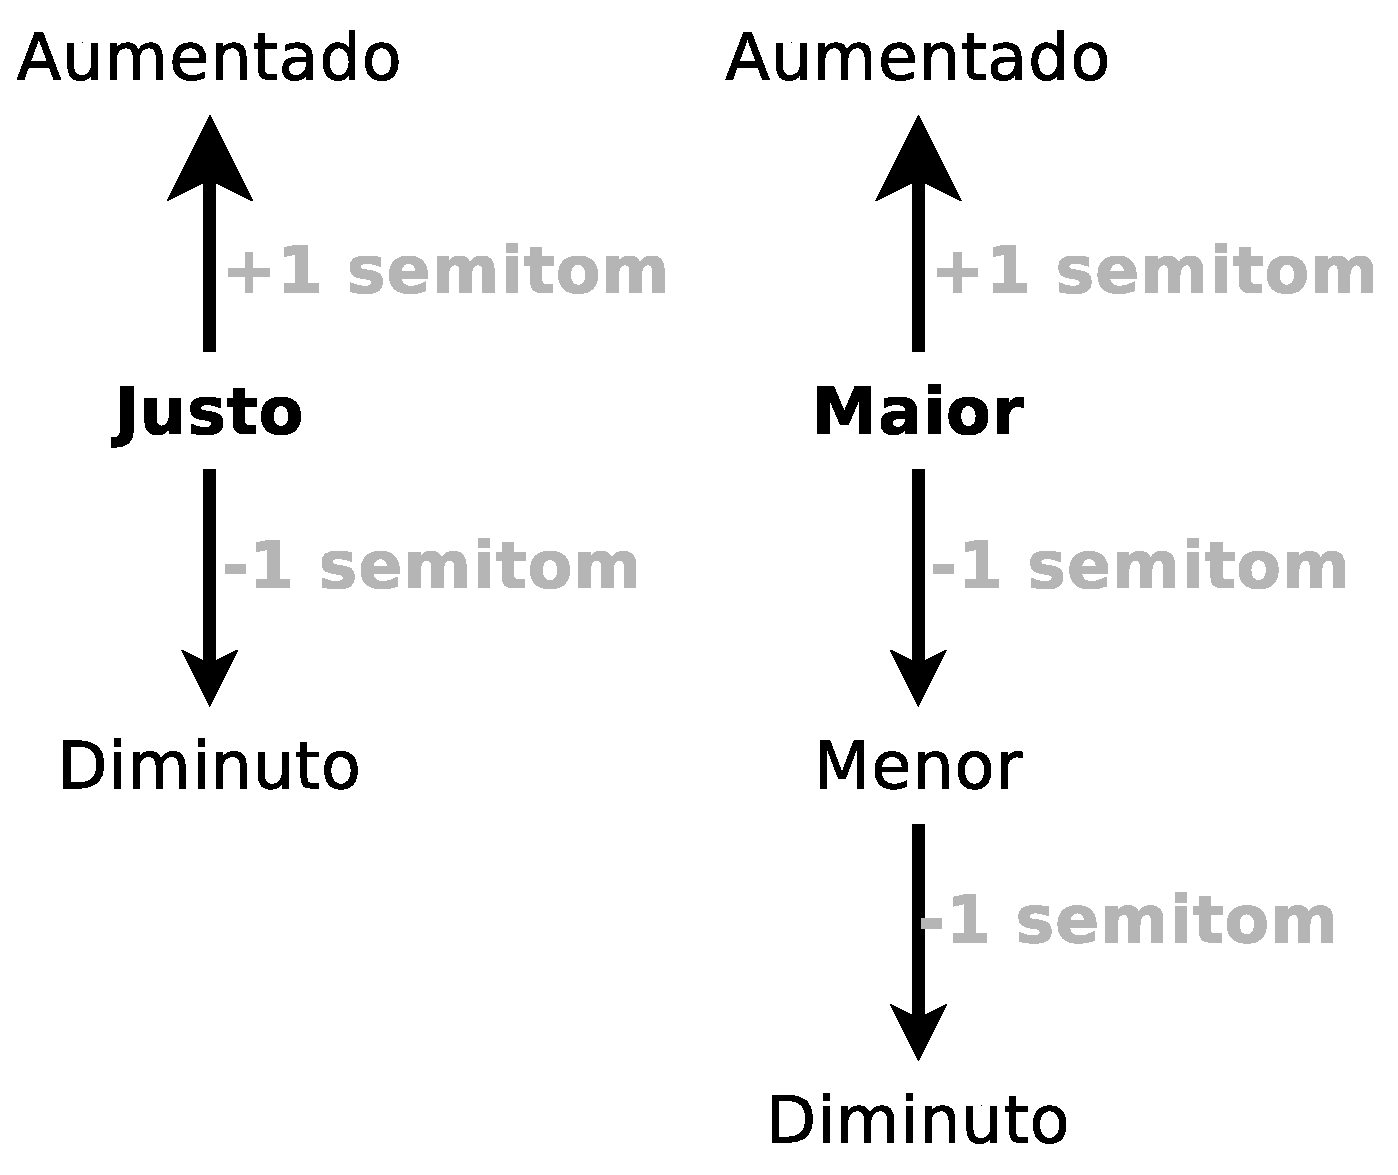
\includegraphics[width=0.5\textwidth]{chapters/cap-musica-basica/justo-maior.eps}
  \caption{Intervalos justos maiores e menores.}
  \label{fig:justo-maior}
\end{figure}
Uma forma rápida de lembrar os nomes é seguindo a escala em dó maior, como 
na Figura \ref{fig:abc-justo-maior2}, onde M indica maior e J indica justo. 
\begin{figure}[H]
    \centering
\begin{abc}[name=abc-justo-maior2]
X: 1 % start of header
K: C % scale: C major
V:1 %name="Pauta com clave de fá"   sname="Pauta com clave de fá"
[V:1]  C8 D8 E8 F8 G8 A8 B8 C'8
w:     ~1ºJ ~2ºM ~3ºM ~4ºJ ~5ºJ ~6ºM ~7ºM ~8ºJ
\end{abc}
\caption{Intervalo de uma sétima descendente.}
\label{fig:abc-justo-maior2}
\end{figure}



A Tabela \ref{tab:intervalomelodico2} mostra o número de semitons 
correspondente a cada intervalo \cite[pp. 89-90]{cardoso1973curso} \cite[pp. 72-74]{holst1998abc}.

\begin{table}[h]
  \centering
  \begin{tabular}{|l|l|l|l|}
  \hline
  \textbf{Intervalo} & \textbf{Semitons} & \textbf{Tons} & \textbf{Exemplo}     \\ \hline \hline
  ~                & 0        & 0        & dó \\ \hline
  Segunda menor    & 1        & 1/2      & ré$\flat$ \\ \hline
  Segunda maior    & 2        & 1        & ré        \\ \hline  \hline
  Terça menor      & 3        & 1+1/2    & mi$\flat$ \\ \hline
  Terça maior      & 4        & 2        & mi        \\ \hline  \hline
  \textbf{Quarta justa}     & \textbf{5}        & \textbf{2+1/2}    & \textbf{fá}        \\ \hline
  Quarta aumentada & 6        & 3        & fá$\#$    \\ \hline \hline
  Quinta diminuta  & 6        & 3        & sol$\flat$ \\ \hline 
  \textbf{Quinta justa}     & \textbf{7}        & \textbf{3+1/2}    & \textbf{sol}      \\ \hline \hline
  Sexta menor      & 8        & 4        & lá$\flat$ \\ \hline
  Sexta maior      & 9        & 4+1/2    & lá        \\ \hline \hline
  Sétima menor     & 10       & 5        & si$\flat$ \\ \hline
  Sétima maior     & 11       & 5+1/2    & si        \\ \hline \hline
  \textbf{Oitava justa}     & 12       & 6        & \textbf{dó} \\ \hline
  \end{tabular}
  \caption{Distancia entre intervalos.}
  \label{tab:intervalomelodico2}
\end{table}
